% title: response.tex
% description: Response to eLife Reviewers
% author: twab

% USAGE: 
% to compile this document:
%    R  >>> knitr::knit("response.Rnw")
%    sh >>> pdflatex response.tex





% document setup

\documentclass[11pt]{elife}\usepackage[]{graphicx}\usepackage[]{color}
% maxwidth is the original width if it is less than linewidth
% otherwise use linewidth (to make sure the graphics do not exceed the margin)
\makeatletter
\def\maxwidth{ %
  \ifdim\Gin@nat@width>\linewidth
    \linewidth
  \else
    \Gin@nat@width
  \fi
}
\makeatother

\definecolor{fgcolor}{rgb}{0.345, 0.345, 0.345}
\newcommand{\hlnum}[1]{\textcolor[rgb]{0.686,0.059,0.569}{#1}}%
\newcommand{\hlstr}[1]{\textcolor[rgb]{0.192,0.494,0.8}{#1}}%
\newcommand{\hlcom}[1]{\textcolor[rgb]{0.678,0.584,0.686}{\textit{#1}}}%
\newcommand{\hlopt}[1]{\textcolor[rgb]{0,0,0}{#1}}%
\newcommand{\hlstd}[1]{\textcolor[rgb]{0.345,0.345,0.345}{#1}}%
\newcommand{\hlkwa}[1]{\textcolor[rgb]{0.161,0.373,0.58}{\textbf{#1}}}%
\newcommand{\hlkwb}[1]{\textcolor[rgb]{0.69,0.353,0.396}{#1}}%
\newcommand{\hlkwc}[1]{\textcolor[rgb]{0.333,0.667,0.333}{#1}}%
\newcommand{\hlkwd}[1]{\textcolor[rgb]{0.737,0.353,0.396}{\textbf{#1}}}%
\let\hlipl\hlkwb

\usepackage{framed}
\makeatletter
\newenvironment{kframe}{%
 \def\at@end@of@kframe{}%
 \ifinner\ifhmode%
  \def\at@end@of@kframe{\end{minipage}}%
  \begin{minipage}{\columnwidth}%
 \fi\fi%
 \def\FrameCommand##1{\hskip\@totalleftmargin \hskip-\fboxsep
 \colorbox{shadecolor}{##1}\hskip-\fboxsep
     % There is no \\@totalrightmargin, so:
     \hskip-\linewidth \hskip-\@totalleftmargin \hskip\columnwidth}%
 \MakeFramed {\advance\hsize-\width
   \@totalleftmargin\z@ \linewidth\hsize
   \@setminipage}}%
 {\par\unskip\endMakeFramed%
 \at@end@of@kframe}
\makeatother

\definecolor{shadecolor}{rgb}{.97, .97, .97}
\definecolor{messagecolor}{rgb}{0, 0, 0}
\definecolor{warningcolor}{rgb}{1, 0, 1}
\definecolor{errorcolor}{rgb}{1, 0, 0}
\newenvironment{knitrout}{}{} % an empty environment to be redefined in TeX

\usepackage{alltt}
\usepackage{amsmath}
\usepackage{amssymb}
\usepackage{amsthm}
\usepackage{ragged2e}
\usepackage{caption}
\usepackage{fancyhdr}
\usepackage{graphicx}
\usepackage{titlesec}
\usepackage{blkarray}
\usepackage{csquotes}

% location of figures for this compiled document
\graphicspath{ {./figs/} }


\title{Supplementary Methods and Response to eLife Reviewers\\
\small{Genetic Disruption of WASHC4 Drives Endo-lysosomal Dysfunction and \\
Cognitive-Movement Impairments in Mice and Humans}}


% Authors
\author[1\authfn{0}]{Jamie Courtland}
\author[1\authfn{0}]{Tyler W. A. Bradshaw}
\author[2]{Greg Waitt}
\author[2,3]{Erik J. Soderblom}
\author[2]{Tricia Ho}
\author[4]{Anna Rajab}
\author[5]{Ricardo Vancini}
\author[2\authfn{1}]{Il Hwan Kim}
\author[6]{Ting Huang}
\author[6]{Olga Vitek}
\author[3]{Scott H. Soderling}

\affil[1]{Department of Neurobiology, Duke University School of Medicine, 
Durham, NC 27710, USA}
\affil[2]{Proteomics and Metabolomics Shared Resource, 
Duke University School of Medicine, Durham, NC 27710, USA}
\affil[3]{Department of Cell Biology, Duke University School of Medicine, 
Durham, NC 27710, USA}
\affil[4]{Burjeel Hospital, VPS Healthcare, Muscat, Oman}
\affil[5]{Department of Pathology, Duke University School of Medicine, 
Durham, NC 27710, USA}
\affil[6]{Khoury College of Computer Sciences, Northeaster University,
Boston, MA 02115, USA}

\contrib[\authfn{0}]{These authors contributed equally to this work.}
\presentadd[\authfn{1}]{Department of Anatomy and Neurobiology, 
University of Tennessee Health Science Center, Memphis, TN 38163, USA}

\corr{jlc123@duke.edu}{JC}
\corr{tyler.w.bradshaw@duke.edu}{TWAB}
\corr{greg.waitt@duke.edu}{GW}
\corr{erik.soderblom@duke.edu}{EJB}
\corr{tricia.ho@duke.edu}{TH}
\corr{drannarajab@gmail.com}{DR}
\corr{ricardo.vancini@duke.edu}{RV}
\corr{ikim9@uthsc.edu}{IK}
\corr{huang.tin@northeastern.edu}{TH}
\corr{o.vitek@northeastern.edu}{OV}
\corr{scott.soderling@duke.edu}{SHS}

% page header
\rhead{Response to eLife Reviewers} 

% reduce space above and below equations
\setlength{\abovedisplayskip}{3pt}
\setlength{\belowdisplayskip}{3pt}
\IfFileExists{upquote.sty}{\usepackage{upquote}}{}
\begin{document}

\maketitle


\begin{abstract}

In the review of this manuscript significant concerns were raised by the
reviewers about the validity of our approach to perform protein- and 
module-level inference from our TMT proteomics dataset. Here we address these 
concerns and provide additional description of our stastical approach.

\end{abstract}

\newpage


\section{Reanalysis of SWIP\textsuperscript{P1019R} TMT Proteomics}

At the center of the cogent critique of our manuscript 
were questions about statistical validity of our previously described approach.   
Succinctly, the issue at question is whether or not the R package \texttt{edgeR}
is an appropriate tool for analysis of protein mass spectrometry data.\\

PreviousAt the Plubell et al., 2017
Several tools for analysis of Proteomics data exist.
At least one prior publicTwo previous publications describe the use of edgeR for analysis of TMT

Previously we used a customized workflow \footnotemark{} to preprocess
and normalize the data prior to performing statistical testing using
\texttt{edgeR's} flexible GLM framework. 

At the core of our normalization appraoch is the use of common quality control
(QC) samples, analyzed in technical duplicate in each TMT mixture. The sample 
pool QC sample was formed by combining aliquots of all biological replicates.
This sample therefore is representative biological and technical variation.
Our normalization appraoch, termed IRS normalization, is essential to correct
for 

The most important step in our normalization approach is 
IRS normalization. MS2 random sampling results in identification and
quantification of proteins by different peptides in each MS experiment.
To account for this source of variability, protein measurements are
adjusted by a scaling factor such that the geometric mean of all
internal reference standards are equal (Plubell et al., 2017).
This is essential to account for the stochasticisity of peptide
quantification in MS experiments. Phillip Wilmarth's
\href{https://github.com/pwilmart/IRS_normalization}[GitHub] offers an 
excellent exploration of IRS normalization. \\

However, we failed to thoughougly
consider the overall adequacy of the NB framework for mass spectrometry data. 
Here we reconsider its appropriatness for our TMT proteomics dataset.  \\
Our previous appraoch can be sumamrized as the "Sum + IRS Normalization" method
described by Huang et al., 2020. We summarize proteins as the sum of its
features and use IRS noramlization. A potential weakness of the sum method is
that outlier peptides can strongly influence the summary value. Median-based
methods (median and median-polish) avoid this problem. We examined outliers in a
method described by [xxx]

Statistical inference in edgeR is built on a 
negative binomial (NB), generalized linear model (GLM) framework. 
Therefore, the data are assumed to be adequately described by a NB distribution 
parameterized by a dispersion parameter, $\phi$. \footnotemark{} \\


\footnotetext{ 
	The dispersion parameter can take several forms. 
	\texttt{edgeR} supports three dispersion models: 'common',
	'trended', and 'tagwise'. However, when using \texttt{edgeR's}
	robust quasi-likelihood test methods, only global (i.e. 'common'
	or 'trended') dispersion metrics are appropriate 
	(see \texttt{edgeR::glmQLFit's} documentation).
}


%% figure 1. 
\begin{figure}[ht]
	\begin{fullwidth}
		\begin{center}
		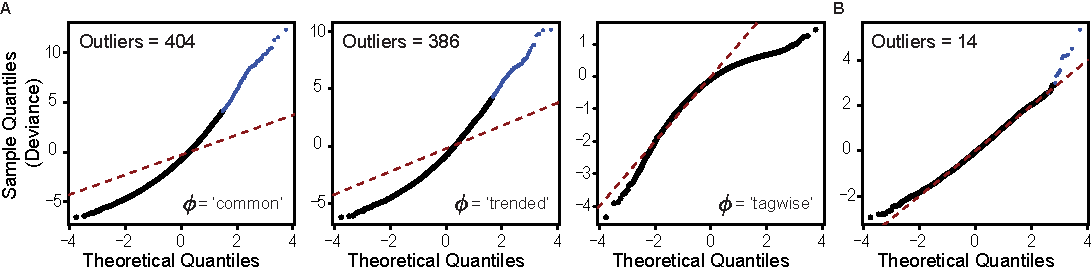
\includegraphics[width=0.9\paperwidth,keepaspectratio]{gof}
		\caption{\textbf{Goodness-of-fit of \texttt{edgeR} (A), and 
		\texttt{MSstats} (B) statistical approaches.} The overall
		adequacy of the linear models fit to the data were assessed 
		by plotting the residual deviance for all proteins as a 
		quantile-quantile plot (McCarthy \textit{et al.}, (2012)). 
		\textbf{(A)} The normalized
		protein data were fit with a NB GLM of the form: 
		\texttt{Abundance} $\sim$ \texttt{Mixture + Condition}.
		Where \texttt{Mixure} is a blocking factor that accounts for
		sources of variablity between experiments. Protein-wise deviance
		statistics were transformed to normality and plotted aganis
		theoretical normal quantiles using \texttt{edgeR::gof}.
		\textbf{(B)}
		The normalized protein data were fit with a linear mixed-effects 
		model (LMM) of the form: 
		\texttt{Abundance} $\sim$ \texttt{0 + Condition + (1|Mixture)}. 
		Where \texttt{Mixture} indicates the random effect
		of \texttt{Mixture}. The residual deviance and degrees of 
		freedom were extracted from the fitted models, z-score
		normalized, and plotted as in (A). Proteins with a significantly 
		poor fit are indicated as outliers in blue 
		(Holm-adjusted P-value $<$ 0.05).}
		\label{fig:gof}
	\end{center}
	\end{fullwidth}
\end{figure}

We evaluated the overall adequacy of the \texttt{edgeR} model by plotting the 
residual deviance of all proteins against their theoretical, 
normal quantiles in a quantile-quantile plot. \textbf{Figure \ref{fig:gof}} 
illustrates the overall lack of fit for the three disperion models fit by 
\texttt{edgeR}.  As an alternative to \texttt{edgeR} we considered 
\texttt{MSstatsTMT}, an extension of MSstats for analysis of TMT proteomics
experiments. \\

\texttt{MSstatsTMT} utilizes a linear mixed-model framework. The strength of 
linear mixed models (LMMs) is in their ability to account for complex sources of 
variation in an experimental design. 

\begin{displayquote}
	In a mixed model one or more covariates 
	are a categorical variable  representing experimental or 
	observational "units" in the data set. 
	[...]
	If the set of possible levels of the covariate is fixed and reproducible 
	we model the covariate using fixed-effects parameters. 
	If the levels that we observed represent a random sample from
	the set of all possible levels we incorporate random effects in the
	model.
\end{displayquote}

A TMT proteomics experiment consists of \texttt{m = 1...M} concatensions of 
isobaric-TMT labeled samples or \texttt{Mixtures}. 
Each TMT channel is dedicated to the analysis of \texttt{c = 1...C}
individual biological or treatment \texttt{Conditions} prepared from one
\texttt{b = 1...B} biological replicates or \texttt{Subjects}. 
A single mixture may be profiled in \texttt{t = 1...T} technical replicate 
mass spectrometry runs. 

We prepared 7 subcellular fractions (BioFraction) from 2 Conditions: 
Control and SWIP\textsuperscript{P1019R} Mutant mice. 
There were 6 Subjects, three bioreplicate Control and 
SWIP\textsuperscript{P1019R} Mutant mice.

\begin{figure}[h]
  \begin{fullwidth}
  \begin{center}
	  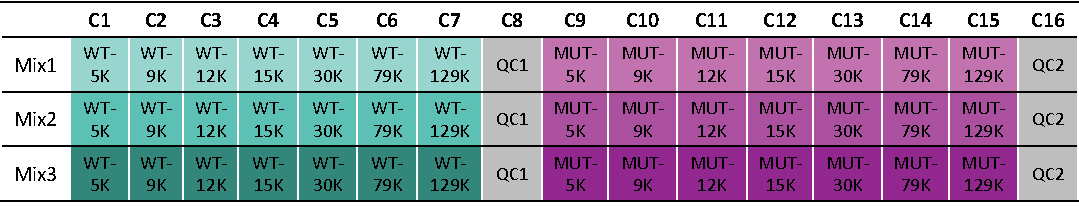
\includegraphics[width=0.9\paperwidth,keepaspectratio]{design}
	  \caption{\textbf{Experimental Design.} We utilized 16-plex
	  TMT tags to label samples prepared from 6 mice.}
	  \label{fig:design}
  \end{center}
  \end{fullwidth}
\end{figure}


\begin{figure}[h]
  \begin{fullwidth}
  \begin{center}
	  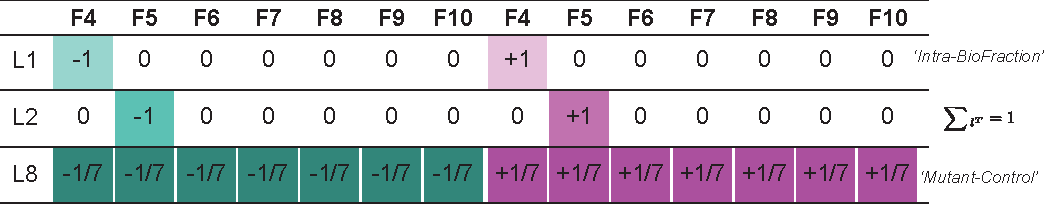
\includegraphics[width=0.9\paperwidth,keepaspectratio]{contrasts}
	  \caption{\textbf{Contrast matrix indicating 'Intra-BioFraction' and
	  'Mutant-Control' comparisons.}} 
	  \label{fig:contrasts}
  \end{center}
  \end{fullwidth}
\end{figure}

In an experiment such as ours with multiple mixtures and biological replicates, 
but no technical replication of mixture (T = 1) \texttt{MSstatsTMT} fits a
linear mixed model of the following form to each protein:

Where Mixture is a mixed-effect and quantifies variation between TMT mixtures.
Condition is a fixed effect (mean = 0) and in our experiment represents the
interaction of terms \texttt{Genotype} and \texttt{BioFraction}. $\epsilon$ 
is a random effect representing both biological and technical variation, 
quantifying any remaining error. \\

\begin{equation} \label{eq1}
	Y_{mcbt} = \mu + Mixture_m + TechRep/Mixture_{m/t} + Condition_c + 
	Subject_{mcb} + \epsilon_{mcbt}
\end{equation}

%\[
%	Mixture_m \sim \mathcal{N}(0,\,\sigma^2_T)
%
%\]

%TechRep/Mixture_{t/m} ~ N(0,\sigma^2_T)
%TechRepMixture the random effect of repeated measruemtns made of mixture nested
%within Mixture. 
%Subject_mcb ~ N(0,\sigma^2_S)
%\epsilon_mtcb ~ N(0,\sigma^2)
%Condition ~ N(0,\sigma^2_T)
%asumed normally distrubted of mean zero


\begin{equation} \label{eq2}
	Y_{mcbt} = \mu + Mixture_m + Condition_c + Subject_{mcb} + \epsilon_{mcbt}
\end{equation}

Where Mixture represents the random-effect of mixture and 
Condition is a fixed-effect and in our experiment is interaction of 
Genotype and BioFraction--the 14 combinations of 7 BioFractions fractions from 
Control and Mutant mice. $\epsilon_{mcbt}$ is the residual error ($\sigma^2$).\\

In our experimental design, we made measurments from seven BioFractions 
from each subject. Thus, we should include the term 
Subject, representing the 6 individual mice or subjects analyzed in our 
experiment. \\


However, in our design \texttt{Mixture} is confounded with the
term \texttt{Subject} -- in each mixture we analyzed all \texttt{BioFractions} 
from a single Control and Mutant mouse. Thus we can choose to account for the 
effect of \texttt{Mixture} or \texttt{Subject}, but not both. 
Assuming Mixture contributes greater to the variance, we drop the term Subject,
and the reduced model is equivalent  to \ref{eq1}. \\

Model based testing of differential abundance between pairs of conditions
is assessed through contrast of conditioned means estimated by fitting the
parameters of the model by REML to obtain $\hat{\beta}$, $\sigma^2$ and
$\hat{V}$.

The degrees of freedom are determined by the Satterthwaite approximation[REF],
and the T-statistic for the contrast is taken to be (lmerTest ref): \\

\begin{equation}
	t = \frac{l^T * \hat{\beta}}{sqrt(l * \sigma^2 * \hat{V} * l^T)}
\end{equation}

$\sigma^2$ is the error from \textbf{Equation} \ref{eq1}.
$l^T$ is a vector specifying a contrast between positive and 
negative coefficients in the model.

Together, the denominator $\sqrt(l * \sigma^2 * \hat{V} * l^T)$ is the 
standard error of the contrast.


\begin{knitrout}
\definecolor{shadecolor}{rgb}{0.969, 0.969, 0.969}\color{fgcolor}\begin{kframe}
\begin{alltt}
\hlkwd{suppressPackageStartupMessages}\hlstd{(\{}
  \hlkwd{library}\hlstd{(dplyr)}
  \hlkwd{library}\hlstd{(data.table)}
\hlstd{\})}

\hlcom{## load SwipProteomics data}
\hlkwd{data}\hlstd{(swip)}
\hlkwd{data}\hlstd{(gene_map)}
\hlkwd{data}\hlstd{(msstats_prot)}
\hlkwd{data}\hlstd{(alt_contrast)}
\hlkwd{data}\hlstd{(msstats_contrasts)}

\hlcom{## formula to be fit:}
\hlstd{fx0} \hlkwb{<-} \hlkwd{formula}\hlstd{(}\hlstr{"Abundance ~ 0 + Condition + (1|Mixture)"}\hlstd{)}

\hlcom{# fit the model}
\hlstd{idx} \hlkwb{<-} \hlstd{msstats_prot}\hlopt{$}\hlstd{Protein} \hlopt{==} \hlstd{swip}
\hlstd{fm} \hlkwb{<-} \hlstd{lmerTest}\hlopt{::}\hlkwd{lmer}\hlstd{(fx0, msstats_prot[idx,])}

\hlcom{# calculate model statistics}
\hlstd{model_summary} \hlkwb{<-} \hlkwd{summary}\hlstd{(fm,}\hlkwc{ddf}\hlstd{=}\hlstr{"Satterthwaite"}\hlstd{)}

\hlstd{df} \hlkwb{<-} \hlstd{model_summary}\hlopt{$}\hlstd{coefficients}
\hlstd{df} \hlopt \hlkwd{as.data.table}\hlstd{(}\hlkwc{keep.rownames}\hlstd{=}\hlstr{"Coefficient"}\hlstd{)} \hlopt \hlstd{knitr}\hlopt{::}\hlkwd{kable}\hlstd{()}
\end{alltt}
\end{kframe}
\begin{tabular}{l|r|r|r|r|r}
\hline
Coefficient & Estimate & Std. Error & df & t value & Pr(>|t|)\\
\hline
ConditionControl.F10 & 7.619237 & 0.1213002 & 17.24812 & 62.81305 & 0\\
\hline
ConditionControl.F4 & 6.711692 & 0.1213002 & 17.24812 & 55.33125 & 0\\
\hline
ConditionControl.F5 & 6.946177 & 0.1213002 & 17.24812 & 57.26434 & 0\\
\hline
ConditionControl.F6 & 7.240695 & 0.1213002 & 17.24812 & 59.69235 & 0\\
\hline
ConditionControl.F7 & 7.321630 & 0.1213002 & 17.24812 & 60.35958 & 0\\
\hline
ConditionControl.F8 & 7.129848 & 0.1213002 & 17.24812 & 58.77853 & 0\\
\hline
ConditionControl.F9 & 6.954883 & 0.1213002 & 17.24812 & 57.33611 & 0\\
\hline
ConditionMutant.F10 & 5.785004 & 0.1213002 & 17.24812 & 47.69163 & 0\\
\hline
ConditionMutant.F4 & 5.405091 & 0.1213002 & 17.24812 & 44.55962 & 0\\
\hline
ConditionMutant.F5 & 5.568104 & 0.1213002 & 17.24812 & 45.90349 & 0\\
\hline
ConditionMutant.F6 & 5.641531 & 0.1213002 & 17.24812 & 46.50883 & 0\\
\hline
ConditionMutant.F7 & 5.633054 & 0.1213002 & 17.24812 & 46.43895 & 0\\
\hline
ConditionMutant.F8 & 5.493008 & 0.1213002 & 17.24812 & 45.28440 & 0\\
\hline
ConditionMutant.F9 & 5.781281 & 0.1213002 & 17.24812 & 47.66093 & 0\\
\hline
\end{tabular}

\begin{kframe}\begin{alltt}
\hlcom{# evaluate goodness-of-fit}
\hlstd{r2_nakagawa} \hlkwb{<-} \hlkwd{r.squaredGLMM.merMod}\hlstd{(fm)}
\hlstd{r2_nakagawa} \hlopt \hlkwd{round}\hlstd{(}\hlnum{3}\hlstd{)} \hlopt \hlstd{knitr}\hlopt{::}\hlkwd{kable}\hlstd{()}
\end{alltt}
\end{kframe}
\begin{tabular}{r|r}
\hline
R2m & R2c\\
\hline
0.935 & 0.949\\
\hline
\end{tabular}

\begin{kframe}\begin{alltt}
\hlstd{contrast} \hlkwb{<-} \hlstd{msstats_contrasts[}\hlnum{1}\hlstd{,]}
\hlkwd{lmerTestContrast}\hlstd{(fm,contrast)} \hlopt \hlstd{knitr}\hlopt{::}\hlkwd{kable}\hlstd{()}
\end{alltt}
\end{kframe}
\begin{tabular}{l|r|r|r|r|r|r|l}
\hline
Contrast & log2FC & percentControl & Pvalue & Tstatistic & SE & DF & isSingular\\
\hline
Mutant.F4-Control.F4 & -0.9075446 & 0.5330916 & 2.5e-06 & -5.986412 & 0.1516008 & 25.99986 & FALSE\\
\hline
\end{tabular}


\end{knitrout}

\end{document}
